\begin{figure}[h!]
    \centering
    \caption{The Effects of \emph{Plan Cuadrante} on Victimization and Reported Crime by Type of Crime}
    \label{fig:figureA8}
    \begin{subfigure}{0.45\textwidth}
        \centering
        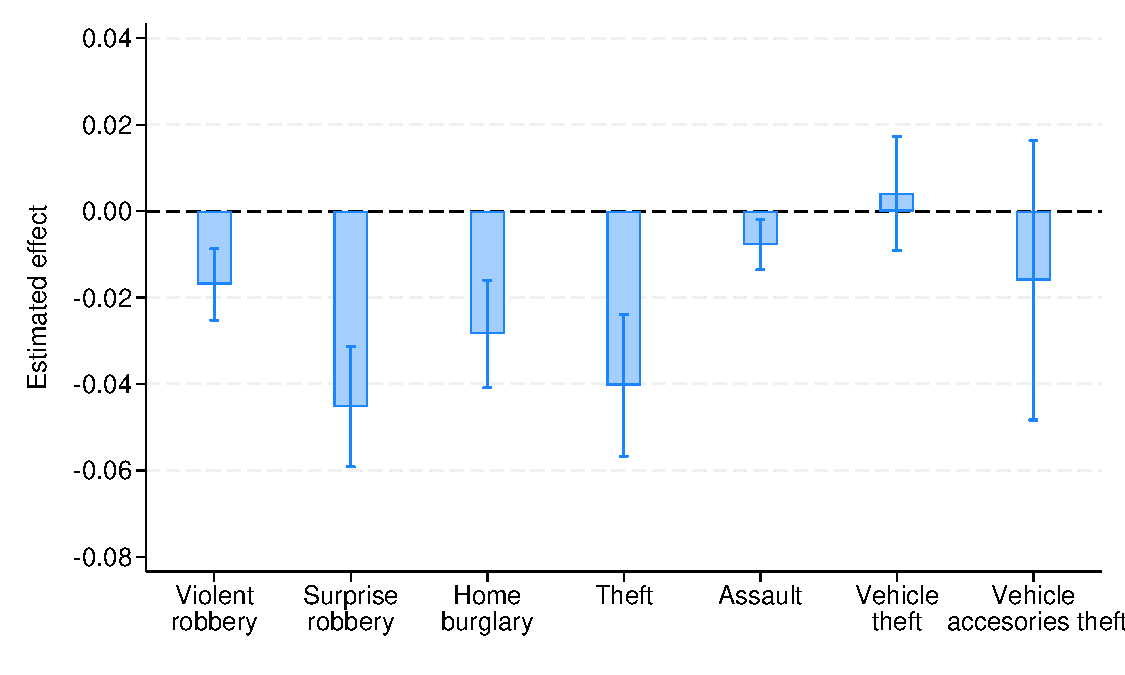
\includegraphics[width=\textwidth]{../manuscript/Graphs/results_typeofcrimes_ENUSC.pdf}
                \caption{Effects on Victimization \\ by Type of Crime}
    \end{subfigure}
    \begin{subfigure}{0.45\textwidth}
        \centering
        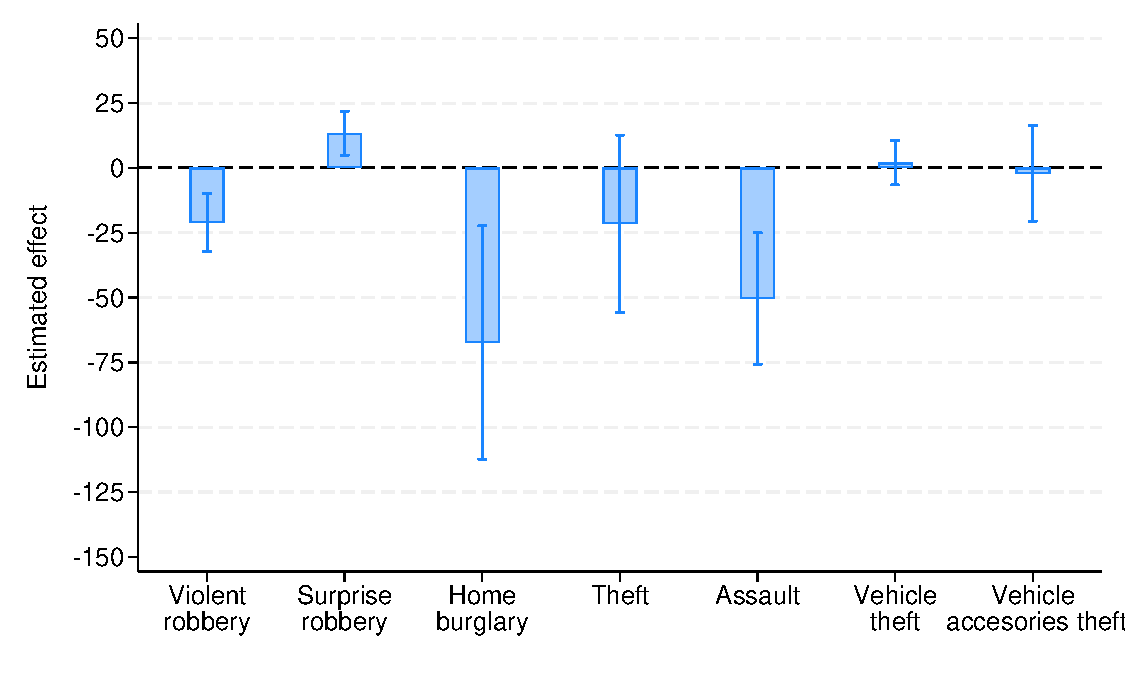
\includegraphics[width=\textwidth]{../manuscript/Graphs/results_typeofcrimes_SPD.pdf}
                \caption{Effects on Reported crime  \\ by Type of Crime}
    \end{subfigure}
    \\[12pt]
    \begin{minipage}{0.99\textwidth}
    \footnotesize Notes: This figure shows the pooled effects of the \emph{Plan Cuadrante} on victimization and number of crimes reported to the police per 100,000 inhabitants by type of crime. The estimation is conducted using the procedure developed in \citet{Callaway} for difference-in-differences with staggered treatment adoption. The graphs display the estimated coefficients and 95\% confidence intervals. Standard errors are clustered at the municipality level using the wild bootstrapping procedure.
    Panel (a) presents the results using victimization data from ENUSC surveys while Panel (b) presents the results using municipality-level administrative data on crime reported to the police provided by the Undersecretary for Crime Prevention. 
    \end{minipage}
\end{figure}